\label{sec:dc_model}

In this chapter we present a range of views of data centres, beginning with some
generic requirements (\Cref{sec:generic_dc}) expressed from two different perspectives: What the data centre is for, and; What
functions are needed?

We then present a more weather and climate view of data centre requirements
(\Cref{sec:wc_requirements}) before considering additional service requirements
around packaging files, and in particular, durability (\Cref{sec:durab1}).

%%%%%%%%%%%%%%%%%%%%%%%%%%%%%%%%%%%%%%%%%%%%%%%%%%%%%%%%%%%%%%%%%%%%%%%%%%%%%%%
\section{Generic Data Centre Requirements}
\label{sec:generic_dc}

At the simplest, a ``data centre'' is a special purpose facility to handle
the production, storage and use of data. Many scientific disciplines make
extensive use of data centres, whether dedicated or shared. Nearly all
such disciplines are facing challenges in planning for the storage and use of
increasing data volumes and the consequential I/O challenges. Much of
what we discuss here will also apply to some or all of:
\begin{itemize}
\item Physics Simulations
\item Particle Physics/High Energy Physics
\item Medicine and Bio-Informatics: Molecular Dynamics
\item Neuroscience and Artificial Intelligence
\item Big Data and Machine Learning
\item Engineering
\item Astronomy
\end{itemize}

Key to understanding and modelling the requirements of the data centre are
to address the degree of specialisation, the application mix, and the impact
of the application mix on workflows and access patterns.

\paragraph{Specialization:}
The amount and nature of discipline specialisation is crucial, and will become
more so in the future as hardware becomes more heterogeneous. In the European
weather and climate community we have to deal with both dedicated and shared
facilities: dedicated to weather, climate, or weather and climate, as well as
shared with other disciplines. For example, in the UK, the academic weather and
climate community share HPC with other disciplines, but have their own dedicated
storage and analysis environment. In Germany, there is a national centre (the
German Climate Compute Center, DKRZ) which provides dedicated compute,
archive, and analysis services, to (primarily) the climate community alone.

Another key facet of specialisation is
whether or not the environment is considered operational, that is,
providing 24x7 services with hot standby --- in which case
extra redundancy is needed, to the point where in the case of the UK Met Office
and the European Centre for Medium Range Weather Forecasting, two separate
computers in two separate computing halls are used to provide such capacity.

In the work we present here, we are going to concentrate on non-operational
environments, but of necessity we address both shared and dedicated data centres.

\paragraph{Application Mix:}

The nature and range of applications supported is crucial. In particular,
from a weather and climate perspective, there are (at least three) particular
application domains to consider: \textit{simulation} (which tends to be I/O intensive
and where poor I/O performance means expensive compute nodes may run idle);
\textit{large-scale analysis} (where data volumes lead to both storage and I/O issues),
and; \textit{archive and restoration} (where discovery, latency, and volume are
all important). Within these broad categories, other important stratification
of application mix include whether or not it is interactive or batch based,
whether high end visualisation is involved (needing specialised hardware),
and whether or not it is (or could be) delivered on virtualised platforms.

In the work presented here, we concentrate primarily on the storage and I/O aspect
of the applcation mix, although of necessity this has impact on all the
computational environments.

\paragraph{Access Pattern:}
In the context of storage, a crucial aspect of consideration is to understand
the access patterns associated with typical workloads. Different access patterns
may have characteristic performance penalties, for example, where patterns can
be characterised as mainly sequential or mainly random, we can model workflow
behaviour.

In general sequential access is faster than random access, but the impact of
storage hierarchy is important. Random access to memory (and storage class
memory) carries little penalty while there is a significant latency and
bandwidth penalty with disk. Tape is prohibitively slow for random access due to
the mechanics of the medium, but after an initial latency, modern tape system
bandwidths can sometimes outperform  disk based approaches .

Often throughput can be improved by appropriate use of caches, but unless this
is automated and the automation system understands the access patterns,
throughput may not meet expectation. This is complicated by the fact that  in
many situations, a pattern obvious to an application is not understandable to
the operating system or the underlying hardware. At the same time, many
applications are ignorant about dynamics in the underlying hardware.

In the work presented here we do not have access to workflow details, so we can
only address the highest level implications of access patterns and caching strategies.

In the remainder of this section, we present a range of functional views
on the structure and requirements of a data centre. The aim is to try to identify
main drivers of costs as the data centre scales towards the exascale.

%%%%%%%%%%%%%%%%%%%%%%%%%%%%%%%%%%%%%%%%%%%%%%%%%%%%%%%%%%%%%%%%%%%%%%%%%%%%%%%
\subsection{Functional View}
\label{sec:dc_func}
\label{sec:dc_services}
\label{sec:dc_discovery}

Originally developed by the Consultative Committee for Space Data Systems
(CCSDS), the Open Archival Information System (OAIS) contains a reference model
[Lavoie] which is now an ISO standard ISO 14721:2012.  While its underlying
purpose is the data centre as an archive, we use it here as a reference for
modelling the data centre's \emph{functional} responsibilities.
Figure~\Cref{fig:dc_arch} shows an extension of the OAIS model, which we use
as a focus for discussing functional requirements.

\begin{figure}[]
  \centering
  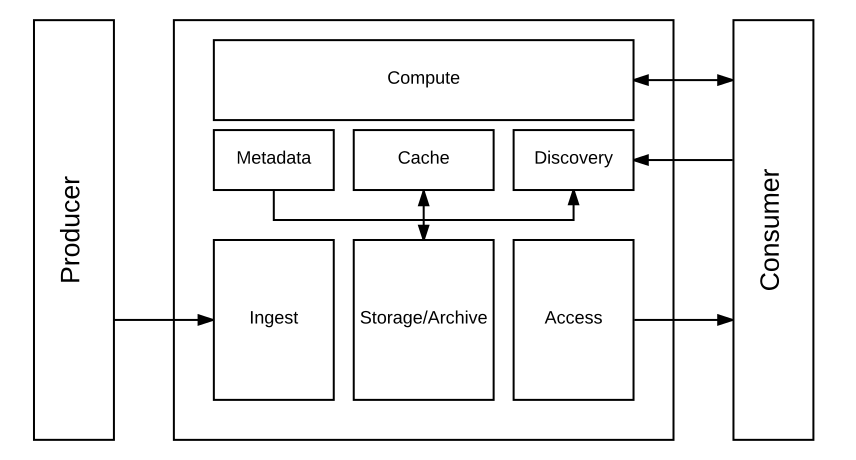
\includegraphics[width=0.6\linewidth]{figures/datacentrefunctional.pdf}
  \caption{Functional architecture of data centre. }
  \label{fig:dc_arch}
\end{figure}

We begin by
concentrating on the relationship between the compute, the storage/archive,
and the network.

% The role of modelling (stochastic and computational) and simulations

% Underlying fabric – covered below (Data Centre Implementation)

% (XXX - fixme: A data centre is not just about data, it is also about compute.  Note distinction in implementing “data intensive” HPC
% compared to “compute intensive” HPC (and supercomputing).)
\paragraph{Compute:}
Very broadly speaking, there are two kinds of scientific computing:
\textit{simulation}, which takes a set of parameters and generates some kind of
output, and \textit{analysis} which takes data and processes it. Received wisdom
has it that analysis generally reduces data volumes (as in statistics, big data,
etc.), whereas simulation increases data volumes. However, in weather and
climate this is not always the case. Many analysis data ``reductions'' create
extra data which has to be differenced from the original data (thus multiplying
up data volumes), and scientific post-processing can often create much more data
than was input (as is the case with an ``afterburner'' approach to producing
diagnostic variables from a weather or climate simulation).  However, there is
one crucial distinction in play: generally simulation compute requires many
(thousands) of compute cores which cannot be idle while waiting for I/O, whereas
analysis compute is generally much smaller, and schedulers can more easily
afford to idle jobs on I/O wait. However, even in analysis compute I/O wait
cannot be excessive, and in fact methods for parallelising I/O are sometimes
even more important in analysis than simulation, and the data centre needs to
provide appropriate hardware support.  Sometimes these two forms of computing
are differentiated by the notions of High Performance Computing (HPC) for
simulation and High Througput Computing (HTC) for analysis computing.

In both cases, coupling data storage with computing resources is necessary: the
alternative of moving large volumes of data repeatedly is expensive and time
consuming, so it is essential to have compute %  (see \Cref{sec:dc_lifecycle})
capability ``close'' to the data (of course it is also essential to be able to
move data around.)

\begin{itemize}
\item Staging: Compute needs to be supported via data staging (job doesn’t
run till data is ready) and ingest (application doesn’t finish till data has
been acknowledged written to storage and/or till the requisite number of replicas
have been created – the durability target has been reached). % (section \ref{sec:durability})
\item Networks: Compute is typically supported on fast interconnect within the data centre,
but the topology can be sensitive to the balance of analysis/simulation and
the need for inter-node communication.  Where simulation and analysis
environments are separate attention to firewall and wide-area network
bandwidth issues is important.
\item Caches:  Both HPC and HTC can benefit from several caching environments
(see Future/Technology) ([Dosanjh],
pp. 35-36, and [Quan et al], pp. 14-18). Application level caching can be
supported with nodes with extra memory, or through NVRAM/SCM (i.e. jobs are
running as a part of the application but their main purpose is to cache data for
fast access by other jobs, or provide dedicated I/O).  Specialised
machines or machine architectures may be needed (or be beneficial) for some
types of applications, thus incurring extra costs.
\item Compute Hardware: The type of compute hardware required may differ
significantly between simulation and analysis, allowing very different
system configuration, quality, and cost to be deployed.
\end{itemize}

\paragraph{Ingest:} Storage can provide different features or different
qualities of service (such as durability and availability), and it is important
to match the user requirements against the features provided by the data centre,
in order to ensure that the correct service is delivered in the most cost
effective manner.  It follows that the user must be able to specify the service
requirements upon ingest; this could happen either via the user specifying
support in policy terms or via directly addressing different parts of the
datastore, e.g.\ via a file path or an object store bucket.

In particular, upon ingest into many types of data centre storage, users ought be
able to:
\begin{itemize}
\item request suitable data storage policy parameters, for example
durability and availability --- via policy terms which might address how
many copies of data were kept and whether it was necessary to have the data
nearline or in cold storage.
\item provide hints as to how data is likely to be recalled, or what parts
of data might be recalled together. If data is stored inefficiently, or
it is necessary to recall larger chunks of the data than are needed, then
recall time may be longer by several orders of magnitude --- which may
be expensive in resources (including potentially human resources).
\item receive notification when the data service goals are reached, e.g. for
durability, that data has been written to the required number of tape copies, s
so that the client can delete its data.
\item employ suitable endpoints to initiate and manage data ingestion (e.g.
browser/command-line/API) via suitable services (e.g. GridFTP etc).
\end{itemize}
(And recognising that data ingestion is something that both happens on the
boundary of a data centre, and within data centre workflows, all
ingestion characteristics also need to be visible to local users.)

In this context, \textit{Recall}, is an important requirement, allowing
users to exploit any storage hierarchy, including from tape. In particular
users should be able to
\begin{itemize}
    \item request data from slower storage and where latency is an issue, be
notified when it is ready, ideally with an estimate prior to recall it of how
long it would take (based on bandwidth and contention),
    \item pre-stage data for batch jobs, so that schedulers can efficiently
    manage compute and storage resources (and so that users don't pay for CPU
    wallclock when the jobs are waiting for the data).
\end{itemize}

\paragraph{(External) Access:}
Users need to be able to export data, and external users may need to access data centre
services to extract data. Suporting export and extraction requires attention to data
discovery, data transfer/service provision, and network bandwidths. In particular,
\begin{itemize}
        \item  Data centres must provide data replication facilities, and
        \item Support high bandwidth network transfers, which may involve
        customised network environments (e.g. see \Cref{sec:dmz}).
\end{itemize}

Such replication and transfer services may need bespoke customisation if the
storage hardware and software doesn't directly support them. For example,
GridFTP \cite{GridFTP}, is a highly efficient open standard data
transfer protocol, which every year transfers hundreds of petabytes of science
data globally, and it forms the foundation of the Globus file transfer services.
Thus, having GridFTP endpoints in the data centre is useful for many customers.
However, when adapting a GridFTP endpoint to
something other than a POSIX filesystem interface, typically some development
work is needed, particularly when good performance is desired (i.e., the service
can take advantage of the striping.)  STFC has put effort into adapting GridFTP
to CEPH, based on original work by CERN, but services can also be bought:
SpectraLogic's Black Pearl supports GridFTP out of the box.  In costing terms,
it becomes a tradeoff between staff (development) or capital (Black Pearl.)

Bespoke services obviously become more expensive, as they need to be integrated
with existing data services and they need to be supported.  Integration is not
necessarily a one-time cost, as upgrades to services may require updates also to
the integration between the services.

\paragraph{Discovery:} Clearly at scale, it is not possible for human intervention
to find and aggregate files for analysis, extraction or replication.  All services
need to be machine interrogatable as to capability and content, and all hardware
needs to support these characteristics. This means in practice that data centre
costs need to include both the software and hardware costs of metadata systems.
It also means that authorisation, authentication and access need to be automated
and data permissions need to be able to be delegated through all levels of the
storage hierarchy.


\subsection{Security}

A data centre has to have security, both physical (access control for authorised
personnel, building security, flood and fire protection) and virtual
(firewall, authentication, possibly at-rest and in-flight encryption).  Of
course, physical security incurs a cost, both in the initial investment and
in operation; likewise staff may need to be vetted and trained in security.  Of
particular importance is that virtual security features do not impede the
performance of data transfer and access: for this reason, unless it is
absolutely required, encryption is switched off for scientific data transfer
(obviously this creates a certain risk of leaking information or a malicious
man-in-the-middle modifying data in flight, but those risks are generally low
and can be accepted without further mitigation).  A data centre must usually
cater to different security requirements,  a typical setup will have mutual
authentication and encryption on the control channel (cf.\ \cite{GridFTP}) and
(only) data channel authentication.

\section{Specific Requirements}
\label{sec:wc_requirements}

Thus far we have looked at generic requirements, albeit from a weather and climate
perspective. Here we focus more on data centre concepts and components of
particular relevance to existing weather and climate.

\begin{figure}
    \centering
    \includegraphics[width=\linewidth]{3rd/workflow-crop.pdf}
    \caption{Characterisation of key elements of weather and climate workflows.
    There are three logical ``data centre'' components, which may or may
    not be physically co-located, and which need to support a range of roles.}
    \label{fig:wc_workflow}
\end{figure}

Figure \ref{fig:wc_workflow} provides a schemtic of the three key
data centre environments from the perspective of weather
and climate workflows:
\begin{enumerate}
    \item An \textit{HPC platform} where the key aspects of the
storage system need to support the fast loading of simulation initial conditions
across thousands of nodes, as well as checkpointing throughout and at the end of
the simulation. Also throughout the simulation is the necessity to write data
out for post-processing and later use: this process generally requires reshaping
of variables, and involves significantly more data handling than the
checkpointing. The storage system associated with this platform generally needs
to support post-processing directly after the conclusion of the run, an activity
which might include multiple software tools and different ways of accessing the
data than were use to write it. Sometimes this post-processing might include
writing most of the data to an archive medium (slower storage tier, such as
tape), for later recall.
    \item An \textit{analysis facility} where users are likely to
    be comparing and contrasting model simulations and observations, and
    so data volumes in some workflows can be significantly larger
    than in any one model simulation experiment. At the same time, software
    is less likely to have inherent parallelisation, although some tasks
    will be able to exploit massive parallelisation in time (for exmaple,
    applying the same algorithm to all timesteps in model output for example).
    This means the storage and I/O systems will likely need to handle even higher
    bandwidths and througput than the HPC platform, and certainly larger
    volumes of accessible data.
    \item An \textit{internet accessible archive} (for example,
    the Earth System Grid Federation, ESGF) from whence users
     can download data to external sites, and where they might potentially
     be able to do either a limited amount of server-side processing, or
     potentially even deploy their own analysis environments on cloud
     computing which has direct acess to the data. Here the storage system
     needs to be well connected through secure interfaces to wide
     area networks, and may have a range of data handling services, from
     GridFTP endpoints, to local provision of ``infrastructure-as-a-service''
     (IaaS) cloud.
\end{enumerate}

There are some distinguishing characteristics of these three environments:
\begin{itemize}
\item The number of users: A relatively small number are responsible for
developing and modifying (tinkering with) models on the HPC platform, with perhaps
hundreds to thousands working in the analysis environment, and with the largest
centres (such as DKRZ and STFC/CEDA) supporting tens of thousands accessing the
outward facing archives. (The number of users will have implication on the
way that storage, services and I/O are organised and scheduled.)
\item The I/O and interconnect subsystems in the HPC platform are likely to need to deal with considerable inter-process communication, while those in the dedicated
analysis facility are more likely to have to deal with simultaneous I/O without
inter-process communication (at least with existing analysis algorithms, future
algorithms may become more complicated as analysis users realise they have
to find new ways of exploiting data parallelism to have acceptable times to
solution - acceptable not only for the user, but also in terms of time
exploiting resources). It is unlikely that much parallelism can be deployed
in the internet archive, unless it is deployed in a public cloud, since most
sites will not be able to deploy enough resources to support large numbers of
users with simultaneous, synchronous computing demands.
\item The amount and complexity of systems to protect users from each other
and from both deliberate and inadvertent data destruction will vary considerably across these domains: on the HPC platform, it can be assumed that all processes
can run with minimal access control beyond constraining ``access to the system''.
By contrast, codes running on an IaaS cloud could do anything, and no write/delete
access should be possible for \textit{anything} running on an untrusted IaaS system. This has implications for the nature of the storage interfaces and their complexity.
\end{itemize}

Of course, in some communities, all three of these environments are deployed
on the same hardware platform and/or in the same machine room. However,
in any modelling of the data centre, one may need to separate out the
systems needed to provide these services (which may also include
replication between environments and storage tiers, as already noted
in the generic reuqirements).

%%%%%%%%%%%%%%%%%%%%%%%%%%%%%%%%%%%%%%%%%%%%%%%%%%%%%%%%%%%%%%%%%%%%%%%%%%%%%
\section{Supporting (Local) Compute Applications}
% moved here from the chapter on related work ...

We have seen the necessity for supporting local compute (as opposed to
primary HPC), whether for post-processing with the HPC, or in dedicated
analysis facilities.

This will have implications for the types of storage necessary:
\begin{itemize}
\item Primary Supercomputing Input/Output, to support:
\begin{itemize}
    \item Input and Output Checkpoint data
    \item Primary Scientific Outputs
\end{itemize}
\item Secondary Input/Output, to support user programmes, but perhaps
with lower I/O bandwidth requirements than primary output.
\item Read Only Primary Data --- data is only read and not updated (although
metadata may be updated),
\item Primary and Secondary I/O storage may support one or both of :
\begin{itemize}
\item Scratch space, and
\item Permanent storage (with assigned durability --- \Cref{sec:durab1}).
\end{itemize}
\item Primary source code storage (ususually with full backup),
\item Append-only storage (e.g. for logs)
\end{itemize}
It may make sense to support these data types differently, depending on
scale, number of users, and typical workflows. Supporting different data
types in different ways is also a logical extension to the general support that
HPC and supercomputing operators give to their application developers: it is in
the interest of both to have applications run as efficiently as possible, and
applications often have to be developed to take the infrastructure into account
(for example, local cache, storage blocks/stripes, parameters for parallel-HDF.)

In addition, metadata storage must be supported not just to aid the application's
use of the data via metadata but also to record the provenance of the derived
data:
\begin{itemize}
\item which algorithms were run and with which parameters,
\item who performed the calculation,
\item which versions of programs and libraries were used,
\item which compute architecture,
\item licences and access permissions for the derived data (which may derive from the licences of the input datasets, possibly in a way which needs to unify different licences on input datasets)
\end{itemize}

\section{Additional Service Requirements}

This section adds further data service requirements, some of which we do not
expect to have implications for initial data centre models such as those
presented in later chapters, but which may both have implications in some future
model which includes service costs and be relevant to other aspects of ESIWACE
exploitability.

\subsection{Packaging and Metadata}
\label{sec:packaging_and_metadata}

 Existing data centres in weather and climate
are primarily based on handling files, which may or may not have internal
metadata content.  However, all centres have developed their own systems which
manage file content, from MASS at the UK Met Office, to MARS at
the European Centre for Medium Range Forecasting. STFC/CEDA expoit bespoke
systems to interface between file based disk, and the CASTOR tape system.
One key part of these systems is that data being migrated between storage tiers
is not necessarily left untouched, tier migration might include:
\begin{itemize}
\item Changes to data granularity, for example
\begin{itemize}
    \item Small files can be packaged up into a shared container (e.g. tar files),
    or
    \item Large files may be pre-chunked or re-chunked to allow optimal
    storage and retrieval along different axes than the original organisation.
\end{itemize}
\item Pool management, where data systems have the notion of pools, datasets
may need to be managed in contigous pools, which may themselves have
specific criteria (e.g. managed for read/write and automatic backup/delete or for write once, two copies, etc).
\item Metadata management, to allow data discovery against both the
original organisation, and the new organisation.
\item Usage Accounting, to support both
\begin {itemize}
\item the use of appropriate use of storage tiers and storage migration (autmatically
making hot data more accessible and moving cold data to cheaper storage but
still available with greater latency), and
\item reporting on data usage, for publication and management metrics.
\end{itemize}
\end{itemize}
All hardware systems will need to support some of these packaging notions,
with consequential implications for software, and data centre costs.

%%%%%%%%%%%%%%%%%%%%%%%%%%%%%%%%%%%%%%%%%%%%%%%%%%%%%%%%%%%%%%%%%%%%%%%%%%%%%%%
\subsection{Durability Implications}
\label{sec:durab1}

It should not come as a surprise that storage with higher durability comes with
a higher cost.  The most basic way of implementing higher durability is LOCKSS --
Lots of Copies Keeps Stuff Safe -- meaning keeping multiple copies of the data,
but keeping $N$ copies reduces the available storage space by a factor $N$.

We discuss this further now, and not in later chapters on cost modelling, since
from the point of view of costing a data centre, we can treat the cost
implications arising from durability requirements as simple multiplicative
factors which impact on storage choices in signifcant ways.

If the loss of a single replica has probability $q$ (in time interval $T$), and we keep $N$ copies,
then the probability of losing all $N$ (equivalent) copies in the same time
frame is simply $q^N$, provided the losses are independent\footnote{Which
is not always a good assumption, for example,
there have been cases where vibrations in disk arrays have caused correlated
disk failures, so it is necessary to actively manage the independence
of the data copies!} of each other.

As a simple model, if the durability ($1-q$) of a single copy of the file is
$0.97$ (in $T$), and a durability of 0.999 is desired, then
$N=\lceil\log(0.001)/\log(0.03)\rceil=2$ copies are needed.
For a durability of $1-10^{-5}$, we would need
$\lceil-5\log(10)/\log(0.03)\rceil=4$ copies. When the time interval
is short, $q$ is relatively small, and $N$ can be small too. When the
time interval becomes long $q$ is inherently greater, and so the durability
falls without extra copies.

Similarly, with many files, the probablility of some data loss scales
at least\footnote{Actually it scales worse than linearly since
many modes of data loss will take out many files at once.} linearly with the
number of files.

It follows from the impact of time intervals on $q$, that the probability
of data loss in any given period $T$ can be reduced by \emph{detecting} the loss
of a copy, within that period, and before further losses occur. That is,
be subdividing the period $T$ into shorter periods $t$, and checking
for file integrity at interval $t$, and where necessary recovering files from
the additional copies.  This has the immediate impact of a direct reduction
on the number of copies needed to maintain acceptable durability for $T$.

This impact can be quantified: for given $q$ and $T$, the probability of
data loss in $t$, $q_t$ is simply $qt/T$. The impact on durability and number
of data copies is straight forward.

Such interval checking can be managed or un-managed. In the latter case it might
occur from normal user data access - when a user attempts to open a primary copy
of data file, and it is found to be bad, a secondary copy can be used (and the
primary copy quietly replaced in the background), but only if it too is bad.
However, this does not provide reliable durability, not only are not all copies
checked (backup copies are only checked if the primary copy is bad), but not all
files are checked. By contrast, if \textit{every} copy of \textit{all} files are
checked for integrity periodically (possibly on a rotation basis), it should be
clear that the durability of the file is improved as the risk of the loss of all
copies of a file in that time is significantly smaller than it would be over
longer time periods.

Periodic detection and repair of data damage can happen in a number of ways.
Live system monioring at the disk and file system level can detect and repair
data loss in many ways, from hardware health monitoring leading to proactive
data  copying (e.g. when drives start showing errors), to the use of RAID
systems which can detect and repair data at the block level.  File systems can
add further automatic fault detection and repair. For example, HDFS replicates
blocks, and it can be configured to replicate blocks across boundaries so the
blocks are not stored in the same drive/array/rack, but copied explicitly to
another for resilience (up to the desired number of copies.)  In the case a
server needs removing from a HDFS infrastructure, instead of the conventional
draining of the server (by moving data from it to other servers), one simply
disconnects it and lets HDFS rebuild the missing copy of the blocks from the
remaining ones.

A similar benefit arises from erasure coding (see definition on page \pageref{para:erasure_codes}). Typically, systems using erasure encoding include
extra complexity, and need more CPU since erasure encoding is handled software
in the storage system - but it can attain higher durability for data since the extra copy overhead is lower.

In any case where automatic rebuilding of data is occurring, the system may be at higher risk of data loss while this takes place, so any system which can minimise this time is advantageous. For example, if it is necessary to drain data
from a server before making additional copies, or rebuilding, this increases
risk over strategies that do not need this initial step.

One key method of minimising durability cost is to used tiered storage, where
lower cost, lower latency media can be used for replicas, since latency is
unlikely to be an issue where recall is in response to automatic periodic
fixity (next section) checking.

The cost of durabilty is obviously smaller if data is compressed or deduplicated
before storage, but the former depends on being able to achieve signficant compression ratios, and has high CPU costs, and the latter is not expected
to work well for weather and climate data - at least at the file level, interesting results have been reported for deduplication of information within data \cite{gmd-10-413-2017}.

\subsection{Durability Requirements}

The importance of durability leads to a set of requirements that are
exposed to system managers (as opposed to internal durability requirements
such as fufilling RAID or erasure encoding related data replication).

\paragraph{Levels of Durability} It must be possible to define and implement different levels of durability.
  \begin{itemize}
      \item It must be possible to communicate available levels to those
      storing data, and it must be possible for such users to choose
      specific levels of durability.
      \item It should be recognised that it may be necessary to manage replicas across sites as well as within a data centre.
  \end{itemize}

  \paragraph{Replication:} Durability may require replication, both within and
  between data centres.
    \begin{itemize}
    \item The placement of the replicas must be aware of the physical location of each replica, in order to maximise risk independence of replicas.
    \item It follows that the replication mechanism must be
    \begin{itemize}
    \item able to ascertain which medium holds a given data set, and
    \item able to determine media which are independent (in terms of risks of failure) of any current location of replicas, and
    \item target the placement of additional replicas to these individual media.
    \end{itemize}
    \end{itemize}

\paragraph{Fixity and Catalogues:} It must be possible to evaluate data integrity.
\begin{itemize}
\item It follows that data must be written and stored in a canonical form which has a well-defined length and can be
  checksummed\footnote{If the data is a file or an object consisting of a sequence of bytes, one would simply checksum
    the data as a sequence of bytes, but other data – JSON, XML, for example – would need to be rendered in a canonical form before being checksummed.}.
  \begin{itemize}
  \item Appropriate checksum technologies should be used (typically file size
  is not enough, tests for bit corruption should also exploit digital hash
  technologies such as MD5 checksums).
  \item Within weather and climate, it is unlikley that provenance fixity
  (e.g. digital signatures) will be necessary.
  \end{itemize}
  \item The length, checksum, storage location of data and replicas, and other relevant metadata, must be stored in a catalogue or other metadata system so this metadata can be preserved and accessed independently.
  \item It should be possible to rebuild the metadata catalogue from the media.
  \item It must be possible to determine the time and status of the most recent integrity check.
  \item It must be possible to check every replica of the data independently.
  \end{itemize}

\paragraph{Preservation Checking:} must be carried out at regular intervals,
which involves evaluating all copies of all data against the fixity catalogue.
This involves:
  \begin{itemize}
  \item Ensuring data is checksummed at ingest.
  \item Evaluating fixity when migrating between storage tiers.
  \item Periodically ``waking up'' data and checking fixity using a pre-defined
  period calculated from the durability requirements.
  \item Monitoring storage media, and taking appropriate action (e.g. monitoring
  disks for bad blocks and/or read/write errors and retiring media with poor
  statistics).
  \item When random failures are found, an investigation and recovery process (that
  is as automatic as possible) should be initiated so that:
  \begin{itemize}
      \item Corrupt data can be replaced,
      \item Statistics of media reliability can be updated,
      \item Where necessary, media can be replace.
      \item Recovery times can be evaluated.
      \item Users and administrators can be appropriately alerted.
  \end{itemize}
  \end{itemize}
